\subsection{GSM8K as a prompt-sensitivity sanity check}
\label{sec:results-gsm8k}

GSM8K behaves as a saturating sanity check rather than a paradigm-ranking benchmark. All four model families reach pass@128 above $0.97$ in the main templated runs, and three of four reach $1.000$, so the benchmark cannot separate paradigms at large $k$. AIME or MATH-Beyond would be needed for that purpose. What GSM8K does separate is prompt format and few-shot count, where the effects are large enough to dominate cross-paradigm differences. Diffusion instruct models lead in zero-shot mode (LLaDA-Instruct pass@1$=0.749$, Dream-Instruct $0.734$ versus Qwen-Instruct $0.534$ and Llama-Instruct $0.488$); $4$-shot prompting essentially closes that gap, raising Qwen-Instruct to $0.789$ and Llama-Instruct to $0.782$. The full $0$-shot, $4$-shot, base, and instruct breakdowns are reproduced in Appendix~\ref{sec:appendix-gsm8k}.

The largest single effect in the entire thesis appears here. Removing the chat template from Llama-Instruct on GSM8K drops pass@1 from $0.782$ to $0.211$, a $57$-point swing on a benchmark on which both prompt modes converge to pass@128$=1.000$. The corresponding row in Table~\ref{tab:gsm8k-instruct-format} therefore demonstrates that two methodologically defensible prompt choices can produce nearly opposite low-$k$ rankings while agreeing at large $k$ once the underlying capability has had enough sampling attempts.

\begin{figure}[!htbp]
\centering
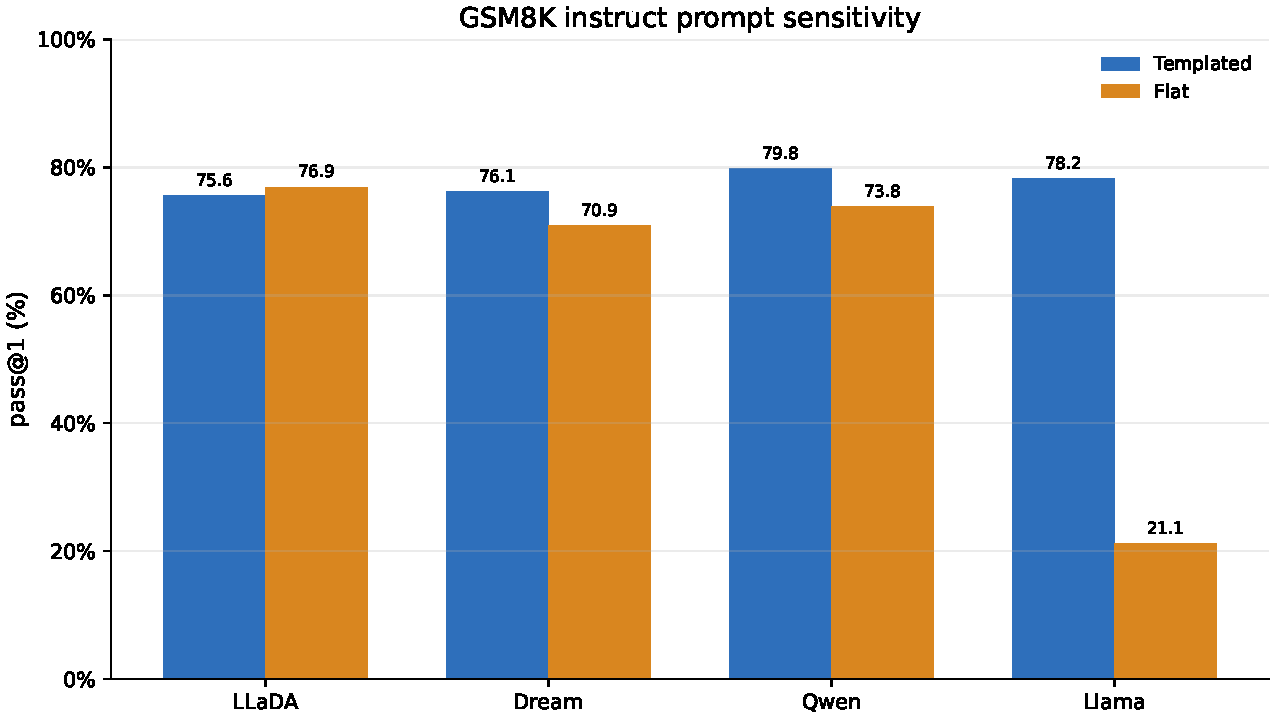
\includegraphics[width=0.78\textwidth]{images/gsm8k_prompt_sensitivity.pdf}
\caption{GSM8K instruct prompt-format sensitivity at pass@1, $n=128$. Llama-Instruct is especially sensitive to flattening, while LLaDA-Instruct slightly improves under the flat format in this run.}
\label{fig:gsm8k-prompt}
\end{figure}

\begin{table}[!htbp]
\centering
\caption{GSM8K instruct templated versus flat pass@k, $n=128$, temperature $=0.7$. The Llama-Instruct row demonstrates that prompt format alone can move pass@1 by tens of points without changing pass@128.}
\label{tab:gsm8k-instruct-format}
\scriptsize
\resizebox{\textwidth}{!}{%
\begin{tabular}{lcccccccc}
\toprule
\textbf{Model / prompt} & \textbf{1} & \textbf{2} & \textbf{4} & \textbf{8} & \textbf{16} & \textbf{32} & \textbf{64} & \textbf{128} \\
\midrule
LLaDA-Instruct templated & 0.756 & 0.852 & 0.905 & 0.942 & 0.968 & 0.982 & 0.990 & 0.992 \\
LLaDA-Instruct flat      & 0.769 & 0.861 & 0.908 & 0.937 & 0.955 & 0.966 & 0.974 & 0.984 \\
Dream-Instruct templated & 0.761 & 0.844 & 0.893 & 0.926 & 0.950 & 0.966 & 0.975 & 0.977 \\
Dream-Instruct flat      & 0.709 & 0.820 & 0.885 & 0.922 & 0.947 & 0.965 & 0.978 & 0.984 \\
Qwen-Instruct templated  & 0.798 & 0.875 & 0.918 & 0.945 & 0.965 & 0.981 & 0.993 & 1.000 \\
Qwen-Instruct flat       & 0.738 & 0.829 & 0.889 & 0.931 & 0.959 & 0.976 & 0.984 & 0.984 \\
Llama-Instruct templated & 0.782 & 0.882 & 0.942 & 0.977 & 0.994 & 0.999 & 1.000 & 1.000 \\
Llama-Instruct flat      & 0.211 & 0.365 & 0.569 & 0.777 & 0.921 & 0.983 & 0.998 & 1.000 \\
\bottomrule
\end{tabular}}
\end{table}

GSM8K therefore enters the thesis as an evaluation-protocol stress test: it shows that prompt format and few-shot count are not implementation details but first-class experimental variables, and it justifies reporting both prompt modes for the more diagnostic Countdown and Trip Planning benchmarks that follow.
